% Gerado automaticamente. No preambulo do documento use:
% \usepackage{pgfplots}
% \pgfplotsset{compat=1.18}
\definecolor{plotblue}{HTML}{2563EB}
\definecolor{plotorange}{HTML}{D97706}
\definecolor{plotgreen}{HTML}{059669}
\definecolor{plotpurple}{HTML}{7C3AED}
\definecolor{plotgray}{HTML}{374151}
\definecolor{plotred}{HTML}{DC2626}
\definecolor{plotteal}{HTML}{0F766E}
\definecolor{plotslate}{HTML}{64748B}

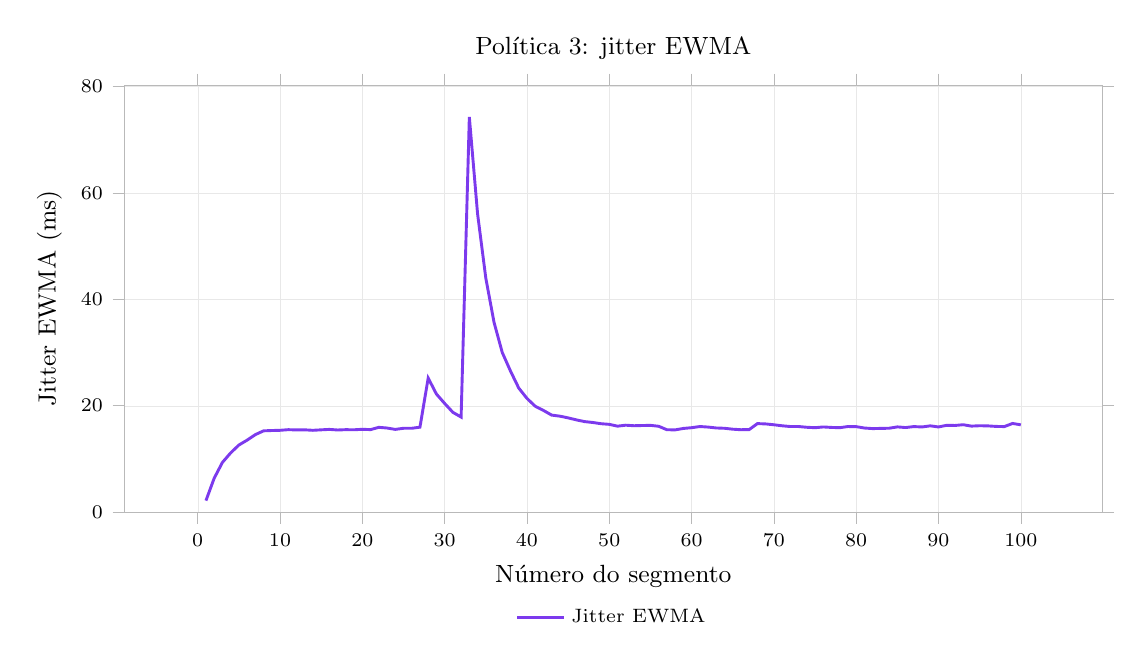
\begin{tikzpicture}
\begin{axis}[
    title={Política 3: jitter EWMA},
    xlabel={Número do segmento},
    ylabel={Jitter EWMA (ms)},
    width=14cm,
    height=7cm,
    grid=major,
    grid style={line width=.12pt, draw=gray!18},
    axis line style={draw=gray!55},
    tick style={draw=gray!55},
    tick align=outside,
    title style={font=\small},
    label style={font=\small},
    tick label style={font=\scriptsize},
    legend cell align={left},
    legend style={at={(0.5,-0.20)}, anchor=north, legend columns=2, draw=none, font=\scriptsize},
    ymin=0,
    ymax=80.2116
]
\addplot+[plotpurple, line width=1.05pt, mark=none] coordinates {
(1,2.15)
(2,6.36)
(3,9.33)
(4,11.12)
(5,12.6)
(6,13.52)
(7,14.56)
(8,15.27)
(9,15.33)
(10,15.37)
(11,15.49)
(12,15.44)
(13,15.46)
(14,15.37)
(15,15.46)
(16,15.54)
(17,15.43)
(18,15.49)
(19,15.47)
(20,15.56)
(21,15.5)
(22,15.93)
(23,15.8)
(24,15.54)
(25,15.75)
(26,15.75)
(27,15.96)
(28,25.19)
(29,22.19)
(30,20.42)
(31,18.75)
(32,17.86)
(33,74.27)
(34,56.08)
(35,43.99)
(36,35.67)
(37,30)
(38,26.51)
(39,23.32)
(40,21.37)
(41,19.9)
(42,19.11)
(43,18.23)
(44,18.03)
(45,17.71)
(46,17.33)
(47,17.01)
(48,16.84)
(49,16.61)
(50,16.49)
(51,16.15)
(52,16.33)
(53,16.23)
(54,16.27)
(55,16.3)
(56,16.13)
(57,15.48)
(58,15.45)
(59,15.72)
(60,15.86)
(61,16.08)
(62,15.98)
(63,15.81)
(64,15.75)
(65,15.58)
(66,15.48)
(67,15.51)
(68,16.63)
(69,16.57)
(70,16.41)
(71,16.22)
(72,16.08)
(73,16.08)
(74,15.94)
(75,15.86)
(76,16)
(77,15.91)
(78,15.86)
(79,16.08)
(80,16.06)
(81,15.8)
(82,15.69)
(83,15.73)
(84,15.76)
(85,16.01)
(86,15.89)
(87,16.07)
(88,16)
(89,16.21)
(90,16)
(91,16.31)
(92,16.28)
(93,16.42)
(94,16.16)
(95,16.23)
(96,16.2)
(97,16.1)
(98,16.07)
(99,16.66)
(100,16.4)
};
\addlegendentry{Jitter EWMA}
\end{axis}
\end{tikzpicture}
